%%%%%%%%%%%%%%%%%%%%%%%%%%%%%%%%%%%%%%%%%
% Journal Article
% LaTeX Template
% Version 1.4 (15/5/16)
%
% This template has been downloaded from:
% http://www.LaTeXTemplates.com
%
% Original author:
% Frits Wenneker (http://www.howtotex.com) with extensive modifications by
% Vel (vel@LaTeXTemplates.com)
%
% License:
% CC BY-NC-SA 3.0 (http://creativecommons.org/licenses/by-nc-sa/3.0/)
%
%%%%%%%%%%%%%%%%%%%%%%%%%%%%%%%%%%%%%%%%%

%----------------------------------------------------------------------------------------
%	PACKAGES AND OTHER DOCUMENT CONFIGURATIONS
%----------------------------------------------------------------------------------------

\documentclass[twoside,twocolumn]{article}

\usepackage{blindtext} % Package to generate dummy text throughout this template 

\usepackage[sc]{mathpazo} % Use the Palatino font
\usepackage[T1]{fontenc} % Use 8-bit encoding that has 256 glyphs
\usepackage[utf8]{inputenc}
\linespread{1.05} % Line spacing - Palatino needs more space between lines
\usepackage{microtype} % Slightly tweak font spacing for aesthetics
\usepackage{float}

\usepackage[english]{babel} % Language hyphenation and typographical rules

\usepackage[hmarginratio=1:1,top=32mm,columnsep=20pt]{geometry} % Document margins
\usepackage[hang, small,labelfont=bf,up,textfont=it,up]{caption} % Custom captions under/above floats in tables or figures
\usepackage{booktabs} % Horizontal rules in tables

\usepackage{lettrine} % The lettrine is the first enlarged letter at the beginning of the text

\usepackage{enumitem} % Customized lists
\setlist[itemize]{noitemsep} % Make itemize lists more compact

\usepackage{abstract} % Allows abstract customization
\renewcommand{\abstractnamefont}{\normalfont\bfseries} % Set the "Abstract" text to bold
\renewcommand{\abstracttextfont}{\normalfont\small\itshape} % Set the abstract itself to small italic text

\usepackage[raggedright]{titlesec} % Allows customization of titles
\renewcommand\thesection{\arabic{section}.} % Roman numerals for the sections
\renewcommand\thesubsection{\thesection\arabic{subsection}} % Big letters subsections
\renewcommand\thesubsubsection{\thesubsection\arabic{subsubsection}} % Big letters subsections
\titleformat{\section}[block]{\large\large\scshape}{\thesection}{1em}{} % Change the look of the section titles
\titleformat{\subsection}[block]{\large}{\thesubsection.}{1em}{} % Change the look of the section titles

\usepackage{fancyhdr} % Headers and footers
\pagestyle{fancy} % All pages have headers and footers
\fancyhead{} % Blank out the default header
\fancyfoot{} % Blank out the default footer
\fancyhead[C]{Real-time DWT processing on mobile platform $\bullet$ Avril 2017 $\bullet$ Projet GTS831} % Custom header text
\fancyfoot[RO,LE]{\thepage} % Custom footer text

\usepackage{titling} % Customizing the title section

\usepackage{hyperref} % For hyperlinks in the PDF
\usepackage{graphicx} 
\graphicspath{ {images/} }

\setlength{\droptitle}{-4\baselineskip} % Move the title up

\pretitle{\begin{center}\Huge\bfseries} % Article title formatting
\posttitle{\end{center}} % Article title closing formatting
\title{A Comparative Study on Heart and Respiratory Rate Extraction Methods Using an Intelligent Matress } % Title of the article
\author{%
\textsc{S. Otis}\\[1ex]%\thanks{A thank you or further information} \\[1ex] % Your name
\normalsize École de technologie supérieure (ÉTS) \\ % Your institution
\normalsize \href{mailto:samuel.otis.1@ens.etsmtl.ca}{samuel.otis.1@ens.etsmtl.ca}
}
\renewcommand{\maketitlehookd}{%
\begin{abstract}
\noindent Improvements of the vital signs monitoring, at hospital and at home, are increasingly in demand. This is required in order to decrease the quantity of patients' state deterioration and increase the comfort of patients at home. This paper aims to compare four families of signal processing methods normally used in extracting the ballistocardiogram from noninvasive intelligent mattresses. By looking at performance statistics like mean average error and computational speed, we assess the best performing algorithm. Motion artifact is the biggest challenge in to overcome and greatly decreases the efficiency of every method. Results showed us that X was more precise $( x \pm y )$ than any other method, but lacked speed with a run time of x seconds. For real-time purposes and continuous vital signs monitoring, we find that Y is better, even though it has poor robustness with an MAE of. For future studies, it is showed that in-between solutions like Z are most useful.
\end{abstract}
}
\begin{document}
%----------------------------------------------------------------------------------------
%	ARTICLE CONTENTS
%----------------------------------------------------------------------------------------

\maketitle
\section{Introduction}
\label{section:Introduction}
	%Definition of methods for fast copypaste
	Even with todays' means of following patients' Heart Rate (HR) and Respiratory Rate (RR), there remains many false diagnostics or bad monitoring of a patient's state, be it in the hospital or at home. As reported by (Donaldson et al. 2000), the failure to act on results of monitoring or testing and the inadequate monitoring or follow-up of treatment are included in the possible types of medical errors. These errors often lead to a deterioration of the situations and sometimes death. The deterioration of the state of a patient due to suboptimal monitoring of the vital signs, as reported by [(Helfand, Christensen, and Anderson 2011)], calls for continuous vital signs monitoring. By looking at trends in signals like HR and RR, this may help, especially at night, to monitor the patients health. That is, it is possible to predict and/or detect particular cardiac or respiratory events leading to deterioration of one's state.
	
	%Ballistocardiogram------------------------------------------------------------------------------------------
	One of the best ways of acquiring HR in a non-invasive way is through the Ballistocardiogram (BCG). The BCG measures the ballistic forces generated by the heart, that is, the mechanical response of the body when the heart ejects the blood into the vascular tree. This technique has been used since the late 19th century \cite{gordon_certain_1877}, but failed to justify its usefulness. 
	%Still, it has awakened much interest for bridging a gap in basic Electrocardiogram (ECG), that is, a new information about the actual state of the vascular tree and the pumping effect of the heart \cite{singewald_ballistocardiography:_1954}. 
	%Lately, with the improvements of signal processing tools and technological advancements, the interest for the BCG was renewed. It is a most useful tool to obtain important information on the cardiac cycles as well as on the respiratory dynamics, while being unobtrusive. 
	Still, analogous to the ECG, which possesses the so-called QRS complex describing the high-amplitude shape of the electrical stimulations during systolic and dystolic cycles, the BCG possesses the IJK complex, as seen in figure \ref{fig:bcg}. It is thus possible to extract information such as the JJ intervals to characterize the heart rate. 
	One of the difficulties in analyzing such signals lies in getting rid of the motion artifacts, that is, when a person moves its body while trying to record the BCG. 
	
	\begin{figure}
		\hfill\includegraphics[width=4cm]{bcg.eps}\hspace*{\fill}
		\caption{ Shape of a BCG signal and the IJK complex.}
		\label{fig:bcg}
	\end{figure}
	
	%Sensors
	Most of the sensors used to detect the BCG, and analogously the RR, are intelligent matresses. These mats are sensible enough to detect micromovements belonging to vital signs such as HR and RR.
	An interesting sensor newly developed is the microbend fiber optic sensor (FOS). FOSs are a new way of acquiring the mechanical activity of the human body through the intensity attenuation of the light in response to an external displacement during the transmission\cite{udd_overview_1995}. Figure \ref{fig:fos} demonstrates the configuration of the microbend FOS. They have been thoroughly used due to their high sensitivity and lower cost of production. 
	
	\begin{figure}
		\hfill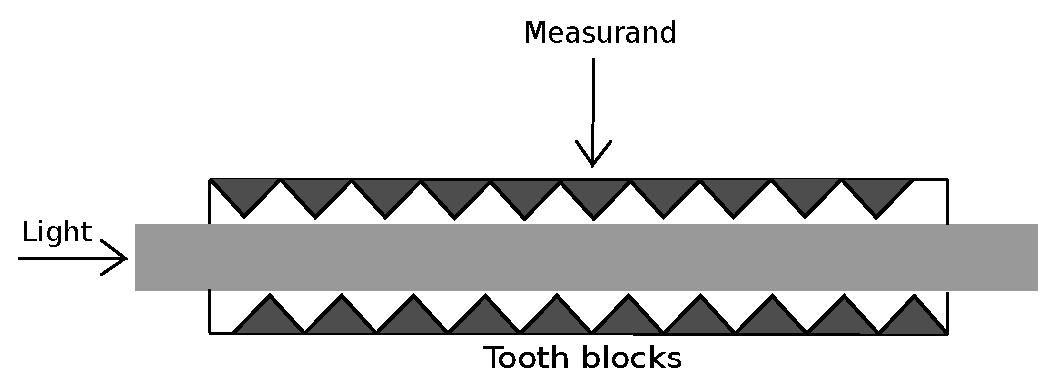
\includegraphics[width=6cm]{fos.eps}\hspace*{\fill}
		\caption{ Microbend FOS principle. The light passing through the microbend FOS is modulated by the deformations in the optical fiber due to the displacement of the microbenders.}
		\label{fig:fos}
	\end{figure}
	%More precisely, the microbend theory is used for building special types of FOS. Microbending of the optical fiber causes an attenuation of the light transmited through it, as per critical angle property \cite{udd_overview_1995}. Multiple pairs of microbenders, when displaced due to physical perturbation, squeezes the fiber. This causes more intensity loss in the cladding region of the optical fiber and increases in function of the pressure exerted on the sensor. 
	%Other known sensors are also used. Some mats with inbedded strain gauge or hydraulic sensor were developed and were mostly used to monitor respiratory and cardiac activity as well as body movements.  Piezoelectric sensors with PVDF or EMFi material designed in a mat also monitored such signals. 
	
	The key to extracting important information from the raw pressure-sensitive signal of the FOS mattress lies in well-known processing tools. Many sources of noise may pollute the signal, be it the "flicker" noise (1/f noise or pink noise) coming from the electrical equipment, the surrounding power line interference at 50 Hz or 60 Hz, depending on the location, or the motion artifact noise. The biggest sources of noise are the motion and breathing artifacts, interfering with the measurements when the subject does even the smallest motion. To find the BCG in all these sources of noise, many signal processing tools from simple to complex ones are used.
	%DSP---------------------------------------------------------------------------------------------------------
	As it is possible to see in section \ref{section:LR}, most of the processing tools used in the literature can be classified in four big families. The first we evaluate is the Wavelet Transform (WT).
	%Wavelets----------------------------------------------------------------------------------------------------
	The WT is often used for signal denoising as well as for feature extraction. Its strength relies in its ability to split the signal into multiple frequency components. That is, we gain a spectro-temporal representation of this signal. The transform operation actually convolves the signal through bank of lowpass and highpass filters, thus giving detail and smooth coefficients, representative of coarse and finer scale phenomenons. 
	%It is possible to go deeper in the decomposition levels by reapplying the passage into the filters to gain detail coefficients at finer scales. Compared to the Fourier transform, the wavelet transform is able to detect discontinuities in the signal without generating too much coefficients to characterize it. 
	%------------------------------------------------------------------------------------------------------------
	%EMD---------------------------------------------------------------------------------------------------------
	Another useful of tool is the empirical mode decomposition (EMD). It is a modified method derived from the Hilbert Transform called the Hilbert-Huang transform \cite{huang_empirical_1998}. This method decomposes a given signal in finite and smaller 'intrinsic mode functions'(IMFs). It then allows to see instantaneous frequencies as a function of time.
	%------------------------------------------------------------------------------------------------------------
	%Cepstrum----------------------------------------------------------------------------------------------------
	Last but not least, the cepstrum is a long known processing technique often used for speech processing \cite{oppenheim_frequency_2004}, based in the domain of the quefrencies. Still, its usefulness in terms of heart rate and breathing rate extraction is undeniable. The cepstrum is the inverse Fourier transform of the logarithmic spectrum of a signal. With this representation, we can uncover the fundamental periods of a signal, that is, the time occurence of certain signal such as heart and breathing rate.
	%-------------------------------------------------------------------------------------------------------------
	
	%Goal of the paper--------------------------------------------------------------------------------------------
	In this paper, we aim to implement four methods \cite{sadek_automatic_2015}\cite{sadek_continuous_2017}\cite{bruser_adaptive_2011}\cite{zhu_heart_2014}, using an FOS mat, that proved effective in extracting the heart and/or respiratory rate and are often used and/or referenced in the literature. Then, these methods will be compared across different performance metrics.

\section{Litterature Review}
\label{section:LR}
	\subsection{Sensors}
	\label{subsection:LR-Sensors}
	%Sensors--------------------------------------------------------------------------------
		Lots of efforts are directed toward the use of FOS for ballistocardiograms and other biomedical signals. Lau and al. \cite{lau_intensity-modulated_2013} developed a microbend fiber optic sensor able to measure the force exerted on a sensor mat. This extremely sensitive mat was used in an MRI environment from the perspective of real-time measuring and recording of the breathing rate. The raw data went in a bandpass filter stage and a peak detection algorithm to retrieve the breathing rate of the patient. The novel sensor showed successfull results in acquiring an MRI in a respiratory-gated acquisition, thus preventing respiratory physiological noise from patients in the MRI.Chen and al. \cite{chen_portable_2012} also used a microbend FOS to extract the BCG from healthy subjects by applying band pass analog and digital filtering to the recorded signal. The BCG is measured on the back of a patient sitting on a chair. They used a NI acquisiton card and a running version of Labview on a computer to acquire the signal and filter it. Analogic filtering was successfully applied directly on the prototype to further reduce the cost of their system. Sadek and al. \cite{sadek_automatic_2015} used a Fiber Bragg Grating Sensor (FBG) to sample the BCG from ten subjects from under a thin bed sheet.  Dziuda and al. \cite{dziuda_monitoring_2012} used  an FBG to extract the breathing rate as well as the heart rate from a healthy subject. The sensor is placed between the back of the subject and the back of a chair and undergoes filtering, averaging and referencing with an ECG. Other than FOS sensor, researchers used other sensor type as described earlier. Pino and al. \cite{pino_noninvasive_2015} retrieved the heart rythm using an EMFi piezoelectric sensor.
	
	\subsection{Digital Signal processing}
	\label{subsection:LR:DSP}
	%Signal preprocessing--------------------------------------------------------------------
		\subsubsection{Wavelet transform}
		%Wavelets
		Aiming to record vital signs in a non-obtrusive way, Postolache and al. \cite{postolache_vital_2007} transformed the signal with a daubechie 4 wavelet base on eight levels of decomposition. They filtered the target coefficients with a moving average. Their study, based with 10 young subjects, was validated against a reference ECG and a spirometer for the breathing signal. The limit of their study, tough, lies with the use of strictly-sane subjects. 
		Combining Donoho and Johnstone \cite{donoho_adapting_1995} wavelet shrinking method with a symlet 8 wavelet base, Jin and al. \cite{jin_novel_2009} detected the heart rate with a peak searching algorithm. 
		%Validation of their method is only visual using the graphs of their BCG and of the ECG. The study, done with one subject of unknown health state, doesn't give any expression of the heart rate according to time nor deals with the problem of motion artifacts.
		Many other teams also used wavelets with different mother wavelets basis to extract the BCG from the raw recordings. Delière and al. \cite{deliere_ballistocardiogram_2015} implemented continuous wavelet tranform (CWT) with a morlet wavelet base to quantify the ballistocardiogram amplitude modulation induced by respiration (BAMR) in an imposed controlled breathing (ICB) protocol. The BAMR was expressed through the maximum local energy in each cardiac cycle. They could then investigate the heart rate variation (HRV) with the BCG reading rather than with the respiratory sinus arrhythmia(RSA) phenomenon, derived from the ECG. 
		%The results came from four healthy adults and showed good correlations correlation coefficient of 0.8466 between RSA and their new BAMR method. The validation was done between two estimated values, the RSA being calculated with their own algorithm from the RR interval (RRI) of the ECG.
		Sadek and al. \cite{sadek_continuous_2017} implemented the Maximal Overlap Direct Wavelet Transform (MODWT) to extract the BCG signal from a microbend FOS. This method proved far more faster than their precedent method using the CEEMDAN algorithm on the data taken on an FBG sensor mat with little more error on the measurements.They did so with a 8-vanishing moment Symlet  wavelet base. 
		%They validated their study on 50 subjects with a reference ECG.
		
		%Wavelets/EMD
		Pino and al. \cite{pino_noninvasive_2015} compared the EMD and wavelet approach to detect the BCG. They used simple EMD decomposition to extract the BCG. The function modes 2 and 3 contained the heart rate signal but the wavelet approach showed nonetheless better results. Their wavelet approach used a Daubechie 6 wavelet base to extract the detail coefficients which contained the bcg signal. 
		%To validate their research, they used 54 voluntary subjects and a reference ECG. Their study was, though, sensible to motion artifacts, having some heart beats cover results as low as 48\%. That is, 52\% of the heart beats were not detected.
		
		\subsubsection{Empirical Mode Decomposition}
		%EMD
		Pinheiro and al. \cite{pinheiro_online_2010} also decomposed the BCG time series into few components and found the BCG in motionless recordings and were able to recover part of the heartbeat information. It still was unable to recover most of the information when a motion artifact is involved. 
		%They validated on eight subjects, one having a coronary stent, without any ECG reference. Their goal was more oriented toward online computing, achieving an excellent computing time of less than 1 ms per segment. Still, their study was limited by the size of the sample and the lack of ECG validation
		Following the ensemble EMD (EEMD) procedure, Song and al. \cite{song_extracting_2015} extracted the BCG for cardiovascular classification. They used temporal, frequential and non-linear methods to retrieve the heart rate in the BCG and then classify the features with a naive bayes classifier. 
		%They had no ECG reference since their study's goal was to classify diseases. Their best classification result was around 92\%, combining all three heart rate methods. They still had difficulties managing motion artifacts.
		
		Sadek and al. \cite{sadek_automatic_2015} used an enhanced version of the EEMD to extract the BCG from an FBG sensor. This method proved to be reliable. At the ninth decomposition component of the CEEMDAN, they retrieved the heart rate with little error and, together with sensor fusion, they achieved a faster heart rate reading than with EEMD. Moreover, it was more efficient in dealing with motion artifacts and having sensor fusion. 
		%This study, done on 10 subjects, had an ECG reference to validate the results. The backfire of their method is the slow computing time of about 30 seconds for the CEEMDAN algorithm. The subjects were also all healthy, thus having ideal vital signs.
		
		{
		\begin{table*}[ht]
		\centering
		 \begin{tabular}{||c c c c||} 
		 \hline
		 Publication & Sensor Type & Target signal & Processing Tool \\ [0.5ex] 
		 \hline\hline
		 \cite{lau_intensity-modulated_2013} &	MFOS & BR & BPF \\
		 \hline
		 \cite{chen_portable_2012}	& MFOS & HR & BPF \\
		 \hline
		 \cite{sadek_automatic_2015} & FBG & HR & EMD \\
		 \hline
		 \cite{dziuda_monitoring_2012} & FBG & BR/HR & BPF \\
		 \hline
		 \cite{pino_noninvasive_2015} & EMFi & HR & WT/EMD \\
		 \hline 
		 \cite{postolache_vital_2007} & EMFi & BR/HR & WT \\
		 \hline
		 \cite{jin_novel_2009} & - & HR & WT \\
		 \hline
		 \cite{deliere_ballistocardiogram_2015} & - & HR & WT \\
		 \hline
		 \cite{sadek_continuous_2017} & MFOS & HR & WT \\
		 \hline
		 \cite{pinheiro_online_2010} & EMFi & HR & EMD \\
		 \hline
		 \cite{song_extracting_2015} & FS & HR & EMD \\
		 \hline
		 \cite{bruser_adaptive_2011} & FS & HR & ML \\
		 \hline
		 \cite{paalasmaa_detecting_2008} & Piezo FS & HR & ML \\
		 \hline
		 \cite{noh_development_2010} & LCS & HR & WT/ML \\
		 \hline
		 \cite{katz_contact-free_2016} & PFS & HR & ML \\
		 \hline
		 \cite{bruser_improvement_2015} & PVDF & HR & CS \\
		 \hline
		 \cite{zhu_heart_2014} & FBG & HR & CS \\
		 \hline
		 \cite{zhu_estimating_2015}	 & FBG & BR & CS \\
		 \hline
		 \cite{kortelainen_multichannel_2012} & PS & HR & CS \\
		 \hline
		 \cite{lee_ballistocardiogram_2015} & LCS & BR/HR & BPF \\
		 \hline
		 \cite{mack_development_2009} & FCP & BR/HR & BPF \\
		 \hline
		 \cite{lydon_robust_2015} & PS & HR & BPF \\
		 \hline
		\end{tabular}
		\label{table*:methods_compared}
		\caption{Summary of other researches in the litterature. MFOS : Microbend Fiber Optic Sensor; FBG : Fiber Bragg-Grating; FS : Force Sensor; PFS : Piezoelectric Force Sensor; PS :  Pressure Sensor; LCS : Load Cell Sensor; FCP : Force Coupling Pad; HR : Heart Rate; BR : Breathing Rate; BPF : Band Pass Filter; WT : Wavelet Transform; EMD : Empirical Mode Decomposition; ML : Machine Learning; CS : Cepstrum}
		\end{table*}
		}
		
		\subsubsection{Machine Learning}
		%Machine learning
		Machine learning, with its recent popularity, has also been applied to extract vital signs from an unobtrusive sensor.
		Bruser and al. \cite{bruser_adaptive_2011} extracted the heart rate with a clustering algorithm.The training phase generated the best prototype heart beat using clustering and kept the prototype amongst all the clusters which represented best the heart beat. They then used cross correlation between the rest of the signal and the prototype to find all the heart beats. Euclidian distance was also a mean to find the heart beats as well as the heart valve signal (HVS). 
		%They performed the validation on 16 healthy subjects, aiming their research to ideally detect cardiac arrhythmia. An lead-I ECG reference was used and they reported a heart beat coverage of nearly 96\% with only 1.79\% error. Nonetheless, the study is limited by the need to perform the training phase manually each time. They also have only one case of arrhythmia, which is not enough to pronounce results in this direction. 
		Paalasmaa and Ranta \cite{paalasmaa_detecting_2008} used also a clustering algorithm but with an ideal signal which they generated. 
		%Their detection rate of less than 50\% was well below the one of Bruser and al. [2011]. The study was still validated with and ECG reference and 3 subjects. They yet have to find a better way of isolating the right cluster for representing the heart beat. As of now, they select the cluster with the biggest density. 
		Following them are Noh and al. \cite{noh_development_2010}, who developed a portable module for heart rate detection. They preprocessed the raw signal coming from the sensor mat with a daubechie 4 wavelet base and applied a layer of template mathcing on top of it to increase robustness. The template is generated from the correlations in the input signal. They use the wavelets to filter and run a peak detection algorithm. The heart beats are also found by doing correlation again between the template and the rest of the input signals. The wavelets alone showed an efficiency of 94\% in detecting the heartbeats of a sample of 10 students. With the ML layer, they increased the detection rate to 98\%. 
		%The study is referenced with a lead-I ECG, but the authors do not give enough details as to how the template is generated. Moreover, all signals are ideal since all the subjects are healthy. More simple ML methods were used and proved efficient. With a simple logistical binomial regression, Katz and al. \cite{katz_contact-free_2016} classidied interbeat intervals (IBI). Done on 14 healthy subjects and validated with and ECG lead-II, they had a maximum error of 20.75 ms on the duration of the IBI between two beats. They aim to base future works on arrhythmia, though this topic is very lightly taken on.
		
		
		
		\subsubsection{Cepstrum}
		%Cepstrum
		The cepstrum, as described before, has been applied with good results to estimate the heart rate. Bruser and al. \cite{bruser_improvement_2015} made the mean of the spectrum recorded on different sensors with a sliding window and then converted it to the cepstrum domain. With a simple peak detection, it was possible to find back the heart rate. Their BedS method had a deviation of 150 ms in the IBIs.
		Zhu and al. \cite{zhu_heart_2014} used the same approach by extracting the cepstrum from a sliding window algorithm. They then filtered the cepstrum to make easier finding the heart rate peak. They achieved an error around 1\% for the whole recordings. 
		In another study, Zhu and al. \cite{zhu_estimating_2015} detected the breathing rate using a similar approach but with many multiresolution windows on three mats containing 6 sensors each. Their results all had a very small error below 1\%.
		Kortelainen and al. \cite{kortelainen_multichannel_2012} extracted the heart and breathing rate using many windows containing two beats per window. Then, by applying the cepstrum on these windows and looking at the difference between two consecutive cepstrums, they achieved 0.4\% error on the heart rate and 1.5\% error on the breathing rate.
		
		\subsubsection{Other methods}
		Lots of others methods were developed using simpler processing tools. Lee and al. \cite{lee_ballistocardiogram_2015} applied heart and breathing rate detection on two babies with a simple band pass filter and moving average window. T
		%hey detected 95\% of the beats in average with an error of 1.53\%. A peak detection algorithm retrieved the heart beats.
		%, with an ECG reference and respiratory sensor. 
		%This study has a really small amount of subjects for validation though, and was not tested against motion artifacts. 
		Mack and al .\cite{mack_development_2009} used an infinite impule response (IIR) bidirectionnal filter and detected local peaks in the signal. 
		%With a special peak searching algorithm, they isolated all probable peaks and derived the heart and breathing rate on 40 subjects with ECG and RIP belt. 
		%They were interested about sleep apnea too, but had no automatic detection of apnea phases during sleep monitoring. 
		Lastly, Lydon and al. \cite{lydon_robust_2015} used a band pass filter and a short moving average window to extract the energy from 0.3 s segments. They computed the heart rate with these windows and adjusted the last computed heart rate with a moving average of the estimate. 
		%Their method had a maximum of 1.85\% error. 
		%One group of three young subjects and another of four elderly subjects helped validate their study. The reference was a piezoelectric finger sensor. Motion artifacts and posture were not included in the results.
		It is possible to view, at table \ref{table:methods_compared}, a summary of the important aspects in the literature concerning the extraction of vital signs from an intelligent mattress. 

\section{Methodology}
\label{Section:Methodology}
	\subsection{Hardware description}
	\label{subsection:Methodology:HD}
		Following the aim of this study, the sensor was fixed against a regular office chair back, as visible in 	figure \ref{fig:chair}. The system used for collecting data includes an small FOS mat and a module to 	gather analogic data coming from the mat. The raw data is sampled at 50 Hz by the module. For reference purposes, this study uses a new acquisition mean under the form of an intelligent textile. The Hexoskin, a training shirt able to capture the HR and RR, is worn by the subject during the whole experiment. Figure \ref{fig:ecgbcg} shows an example of BCG signal and ECG reference signal. The whole data is processed in MATLAB R2017a with [insert operating system and CPU specs].
	
	\begin{figure}
		\hfill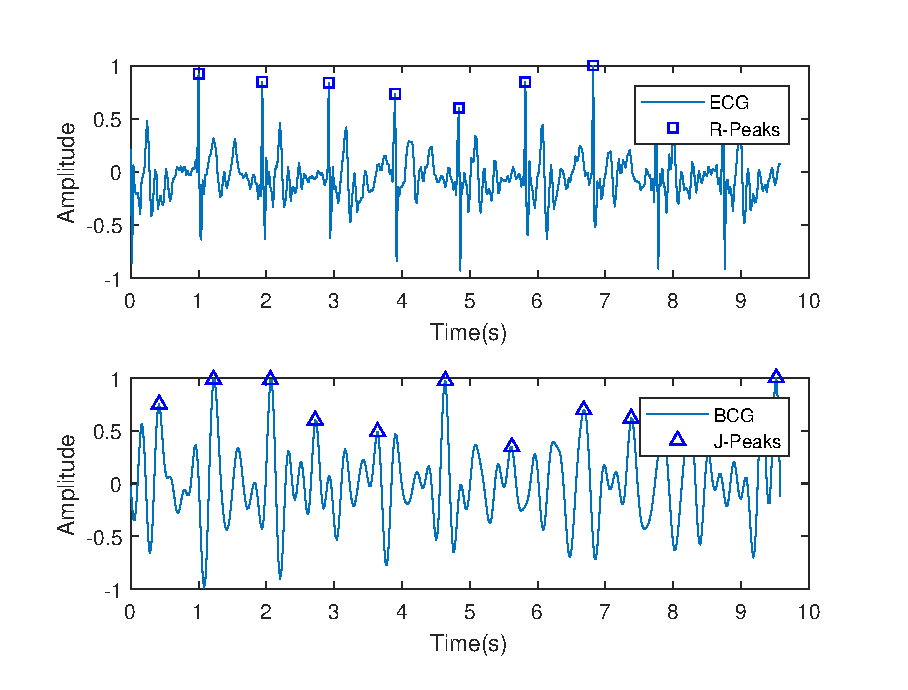
\includegraphics[width=7cm]{ECGvsBCG.eps}\hspace*{\fill}
		\caption{An example of ECG reference signal with R-Peaks, compared to BCG signal with J-Peaks}
		\label{fig:ecgbcg}
	\end{figure}
	
	\subsection{Experimental setup}
	The results are gathered on 6 subjects, three men and three women, each between 20 and 35 years old. The subjects were gathered inside the research center using a general invitation. Each subject is asked to sit and stay still on the chair during the whole procedure. After 30 seconds, they are asked to cough to create an event in the signal. This event is used to manually synchronize the mattress signal and the reference signal of the Hexoskin during later processing. They then stay still for 5 minutes on the chair, follow up by holding their breath for 30 seconds and, subsequently,  stay still for another 2 minutes. After, we ask them to cough, first, 10 times by intervals of 5 seconds and then 10 times by intervals of 2 seconds. These events are used for future analysis of the data and better synchronization of the mattress and reference signals. The CHUM medical center's review board has determined that this study poses minimal risk and that it adheres to ethical principles.
	
	\begin{figure}
		\hfill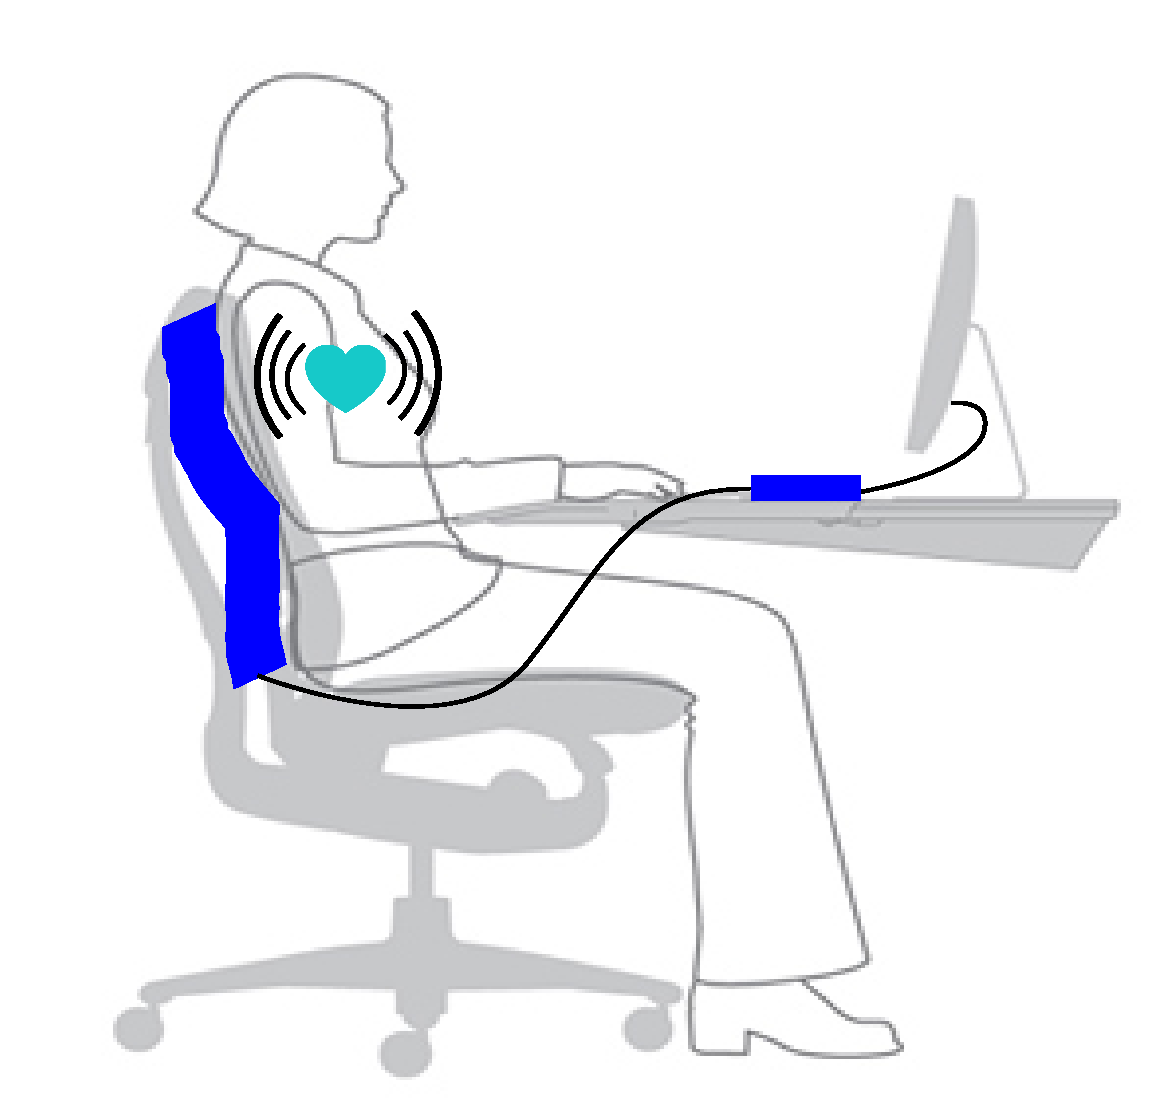
\includegraphics[width=4cm]{chair1.eps}\hspace*{\fill}
		\caption{Experimental setup}
		\label{fig:chair}
	\end{figure}
	
	\subsection{Algorithms}
	\label{subsection:Methodology:Algorithms}
		\subsubsection{Peak searching algorithm}
		For the MODWT, CEEMDAN and Clustering methods, we apply a custom peak searching algorithm using a 10 seconds sliding window. The peak extraction is slightly different for the cepstrum and will be explained at the end of this section. A peak extraction algorithm is necessary since the extraction methods being compared do not extract the heart rate. The BCG signal which still needs to be processed to extract the heart rate from it. The algorithm, which sets normal boundaries fo the HR\cite{zhu_heart_2014}, functions accordingly to the following steps :
	\begin{enumerate}
		\item Peak search the segment of the windowed signal with a default amplitude treshold.
		\item If there are more peaks than a 180 bpm-signal would contain, increase threshold and repeat step 1.
		\item If there are less peaks than a 40 bpm-signal would contain, decrease threshold and repeat step 1.
		\item Determine average J-J interval and extract heart rate
		\item Shift window by 10 seconds and repeat from step 1.
	\end{enumerate}
	Since this paper aims to compare different methods, the peak search algorithm is design assuming that we are isnide normal heart rate tendencies.
		\subsubsection{MODWT}
		The MODWT, having achieved good results in the literature among other wavelets preprocessing methods, is implemented using the built-in toolbox of MATLAB. As stated by Sadek et al.\cite{sadek_continuous_2017}, the 4th level smooth coefficients of the wavelet decomposition is used to extract the BCG. We then apply the peak searching algorithm described earlier.
		\subsubsection{CEEMDAN}
		The literature also possessed many methods making use of the EMD. The CEEMDAN is a derived method which offers better results by dealing with end effects and mode mixing, which degraded the output modes from the standard EMD. This method in particular showed excellent results in extracting the heart rate from still subjects\cite{sadek_continuous_2017}. As recommendedby Sadek et al.[\cite{sadek_automatic_2015}, we set the CEEMDAN parameters according to a noise standard deviation of 0.2, a number of realizations of 100, and a maximum number of iterations of 30. Finally, we apply the same custom peak searching algorithm.
		\subsubsection{Machine learning - Clustering}
		As for the third method, we use the ML method from the paper of Brüser et al.\cite{bruser_adaptive_2011}. The implementation, as described in this paper, starts with the training part. We featurize the 30-seconds training set of the signal and then use Principal Component Analysis (PCA) to reduce the dimensionality of the features. Subsequently, we use a clustering toolbox in MATLAB to create clusters, with the two most important principal component. The resulting feature prototypes which should describe best a heart beat are thus returned. Finally, our implementation uses correlation between the prototype and the whole signal to retrieve heart beats in the complete signal. High correlation values are interpreted as heart beats. We also applied euclidian distance by featurizing the whole signal. Smallest euclidian distances meant that there probably was a heart beat at the related position. Correlation and euclidian distance results both went in the custom peak searching algorithm to extract a heart rate from each of them. We finally merge the two heart rates by averaging each points at the same position.
		\subsubsection{Cepstrum}
		The cepstrum method as seen increased interest in extracting vital signs. Using the research from Zhu et al.\cite{zhu_heart_2014}, we applied a band pass filter 1-10 Hz at -3 dB of attenuation. Thereafter, a sliding 10-seconds window transformed each segment of the signal into the cepstral domain. Another filter was applied to smooth the cepstrum in order to better retrieve the peak of the lag time related to the HR. Each peak was attributed to the central position of the window. Then each window went through a local peak filtering. This filter made sure that each detected local peak was within normal HR limits, which is ~40-180 BPM.\cite{zhu_heart_2014}.
	\subsection{Validation}
	\label{subsection:Methodology:Validation}
	The first measure used to assess the quality of each method is the Mean Absolute Error (MAE). This quantity is used in statistics to measure how close a prediction is to the actual outcome.
	\begin{center}
		\[MAE = \frac{1}{n}\sum\vert y_{i} - \widehat{y_{i}}\vert \] 
	\end{center}
	where 
	\[y_{i} = Actual \]
	and
	\[\widehat{y_{i}} = Predicted \]
	
	The second measure, the Computational Speed, is used to quantify the weight of the operations realized by the system while doing X action. By measuring the system epoch at the beginning and at the end of the algorithm, we can estimate the time it takes to go through the whole algorithm.

\section{Results and Discussion}
\label{section:RD}
	In this work, each methods were applied as described earlier in section \ref{subsection:Methodology:Algorithms}. 
	
	
		\begin{table}[ht]
		\centering
		 \begin{tabular}{cccc} 
		 \hline
		 Subject & MAE (Average) & MAE (Std) & CS \\ [0.5ex] 
		 \hline\hline
		 1 & 12.97 & 8.67 &  \\
		 \hline
		 2 & 11.10 & 5.11 &  \\
		 \hline
		 3 & 25.08 & 9.23 &  \\
		 \hline
		 4 & 17.14 & 5.86 &  \\
		 \hline
		 5 & 15.18 & 10.71 &  \\
		 \hline
		 6 & 7.15 & 4.75 &  \\
		 \hline
		 Mean  & 14.83 & 7.39 &  \\
		 \hline
		\end{tabular}
		\label{table:performance_results}
		\caption{Performance of the MODWT algorithm on all subjects}
		\end{table}
		
		\begin{table}[ht]
		\centering
		 \begin{tabular}{cccc} 
		 \hline
		 Subject & MAE (Average) & MAE (Std) & CS \\ [0.5ex] 
		 \hline\hline
		 1 & 4.76 & 2.13 &  \\
		 \hline
		 2 & 12.66 & 2.76 &  \\
		 \hline
		 3 & 6.09 & 2.32 &  \\
		 \hline
		 4 & 7.15 & 4.37 &  \\
		 \hline
		 5 & 5.20 & 6.02 &  \\
		 \hline
		 6 & 4.71 & 3.21 &  \\
		 \hline
		 Mean  & 6.76 & 3.47 &  \\
		 \hline
		\end{tabular}
		\label{table:performance_results}
		\caption{Performance of the CEPSTRUM algorithm on all subjects}
		\end{table}
		
		\begin{table}[ht]
		\centering
		 \begin{tabular}{cccc} 
		 \hline
		 Subject & MAE (Average) & MAE (Std) & CS \\ [0.5ex] 
		 \hline\hline
		 1 & 9.48 & 2.77 &  \\
		 \hline
		 2 & 2.82 & 1.96 &  \\
		 \hline
		 3 & 4.28 & 2.13 &  \\
		 \hline
		 4 & 1.83 & 1.96 &  \\
		 \hline
		 5 & 7.82 & 7.34 &  \\
		 \hline
		 6 & 9.09 & 3.76 &  \\
		 \hline
		 Mean  & 5.88 & 3.32 &  \\
		 \hline
		\end{tabular}
		\label{table:performance_results}
		\caption{Performance of the CEEMDAN algorithm on all subjects}
		\end{table}
		
		\begin{table}[ht]
		\centering
		 \begin{tabular}{cccc} 
		 \hline
		 Subject & MAE (Average) & MAE (Std) & CS \\ [0.5ex] 
		 \hline\hline
		 1 & 4.44 & 2.85 &  \\
		 \hline
		 2 & 18.85 & 7.70 &  \\
		 \hline
		 3 & 12.57 & 3.19 &  \\
		 \hline
		 4 & 9.11 & 3.20 &  \\
		 \hline
		 5 & 7.83 & 4.48 &  \\
		 \hline
		 6 & 3.25 & 2.60 &  \\
		 \hline
		 Mean  & 9.34 & 4.00 &  \\
		 \hline
		\end{tabular}
		\label{table:performance_results}
		\caption{Performance of the CLUSTERING algorithm on all subjects}
		\end{table}
\section{Conclusion}
In this comparative study, four methods, belonging each to a family of signal processing methods, are used to extract the heart rate from an intelligent FOS mattress. Thus, we put wavelets, empirical mode decomposition, cepstrum and machine learning in competition by examining their mean average error with the reference as well as the computational speed of each of them. Respectively, the methods chosen for each families are MODWT, CEEMDAN, CEPSTRUM by sliding window and clustering. The system is completely non-invasive and the results showed good performances in extracting HR. Each methods extracts in its own way the periodiciy relative to the heart beats, with varying effectiveness. Even if X gives the lowest MAE among all methods, it has poor computational speed. For a real-time purpose, with a run time of Z seconds, Y is more adapted. It is apparent, when comparing each algorithm performance with its counterpart in the literature, that the error increased a lot. This is due to the acquisition protocol that was chosen to record the subjects' vital signs. Many movement artifacts were induced by the actions required in the procedure. Movements artifacts are still the biggest challenge in extracting the BCG from an intelligent mattress. At most, only 5 minutes of each recording is considered clean of movement artifacts. The rest of the recordings are used for future work. This work paves the way in extracting heart rate and other vital signs for future classification of respiratory pathologies. This will help assuming a continuous vital signs monitoring and detection of problems in the patient' state.

%----------------------------------------------------------------------------------------
%	REFERENCE LIST
%----------------------------------------------------------------------------------------
\newpage

\bibliographystyle{plain}
\bibliography{biblio3}
 

\end{document}
